%\begin{tiny}\end{tiny}
\documentclass[12pt,a4paper,titlepage,oneside]{article}
\usepackage{spec_calculator}
\usepackage{rotating}
\usepackage[bookmarksnumbered=true,colorlinks=true,linkcolor=blue]{hyperref}

\title{Calculator}
%TODO: for final Version
\group{
	\groupnr	18
} 
\author{
	\begin{tabbing}
    	\hspace*{4cm} \= \kill
		Harald Glanzer,	\> \matrnr 0727156 {\small harald.glanzer@gmail.com} \\
		\hspace*{4cm} \= \kill
		Stefan Simhandl,	\> \matrnr 0725240 {\small e0725240@student.tuwien.ac.at} \\
	\end{tabbing}
}


\begin{document}

% create titlepage
\maketitle

\tableofcontents
\newpage

\section{Einleitung - funktionale Beschreibung}

Im Rahmen der Laborübung soll ein simpler Calculator entworfen und auf einem FPGA Entwicklerboard implementiert werden. \\
Bezüglich des Funktionsumfanges gibt es die Forderung, dass der Rechner die mathematischen Operationen Addition, Subtraktion, Multiplikation und Division sowie die damit verbundenen Rechenregeln (Punktrechnung vor Strichrechnung, etc.) beherrschen muss. Weiters sollen die letzten 50 Rechnungen gespeichert werden und die Möglichkeit bestehen, diese über die RS232-Schnittstelle des Boards an einen PC zu senden. \\
Das Userinterface besteht dabei aus einem PS/2 Keboard zur Eingabe der Rechenoperationen sowie einem Monitor welcher über die VGA Schnittstelle des Boards angesteuert wird.  Die LVA-Leitung stellt dabei die Module für den VGA-Treiber sowie für die PS/2 - Schnittstelle zur Verfügung.

Der Rechner 

\section{Anforderungen im Detail}

\begin{itemize}

\item Keine Division durch Null(Fehlermeldung)
\item Kein Overflow der Variablen(Fehlermeldung)
\item Keine Leerzeichen innerhalb einer Zahl(Fehlermeldung)
\item Maximale Eingabelänge der Berechnung = 70 Zeichen. Wird diese Anzahl erreicht fährt der Calculator mit der Berechnung der bisher eingegebenen Zeile fort, wenn sich dadurch Syntaxfehler ergeben erfolgt eine Fehlermeldung
\item Zwischen 2 Operatoren ist immer nur ein Operand erlaubt. Ausnahme ist das Zeichen für eine negative Zahl '-'
\item Der erlaubte Zeichensatz ist auf die Ziffern 0-9, +, -, *, /, <ENTER>, <WHITESPACE> sowie <BACKSPACE> - alle anderen Zeichen werden schon bei der Eingabe abgefangen(ignoriert) 
\item Keine Leerzeilen(Fehlermeldung)
\item Keine alleinstehenden Operatoren(Fehlermeldung)
\item Keine alleinstehenden Operanden(Fehlermeldung)

\end{itemize}

\subsection{Aritmetische Ausdrücke}

Es sollen folgende Arithmetische Ausdrücke unterstützt werden:

\begin{itemize}

\item Addition: ERGEGBNIS = ZAHL1 + ZAHL2
\item Subtraktion: ERGEGBNIS = ZAHL1 - ZAHL2
\item Multiplikation: ERGEGBNIS = ZAHL1 * ZAHL2
\item Division: ERGEGBNIS = ZAHL1 / ZAHL2
\end{itemize}


\subsection{Rechenregeln}
Die einzige zu beachtende Rechenregel ist die Regel \textbf{Punktrechnung vor Strichrechnung}. 
Klammerungen sind nicht gefordert und werden folglich auch nicht implementiert.

\subsection{Datentypen}

Als Datentyp soll 'Signed Long' verwendet werden - damit ergibt sich ein Wertebereich von $-2^{31}$ bis \begin{tiny}\end{tiny}$2^{31} - 1$. Overflows bei der Eingabe werden abgefangen, während Overflows welche sich während der Berechnung des eingegebenen Ausdrucks ergeben \textbf{NICHT} abgefangen werden.

\subsection{Userinerface}

Als Userinterface steht einerseits ein Standardkeyboard zur Verfügung, welches mittels PS/2 - Schnittstelle mit dem FPGA-Board verbunden ist. Die Textausgabe erfolgt auf einem Monitor, welcher mittels VGA-Schnittstelle vom Entwicklungsboard angesteuert wird. 
Weiters besteht die Möglichkeit einen Datentransfer zu triggern. Dabei sollen die letzten 50 Berechnungen, welche eingegeben wurden, per serieller Schnittstelle an den PC übertragen werden. Dieser Datentransfer soll entweder per Pushbutton oder nach Empfang eines speziellen Zeichens per RS232 angestossen werden. Wir haben uns entschlossen als RS232 - Trigger das Zeichen 's', ASCII-Code 0x73, zu verwenden.

\subsubsection{Dateneingabe}

Wie gesagt wird hierfür ein PS\/2 verwendet. Als Interface zw. Keyboardhardware und FPGA-Board wird ein Modul von der LVA-Leitung zur Verfügung gestellt. Dieses Modul liefert einerseits den 8Bit-Wert 'data', welcher einen Scancode darstellt, und andererseits ein Steuersignal 'new\_data' welches anzeigt ob ein neuer Scancode zum  Auslesen bereit ist. Abbildung~\ref{fig:ps2timing} zeigt an wann ein neues, gültiges 8Bit - Datenwort gelesen werden darf.

\begin{figure}[!ht]
	\centering
	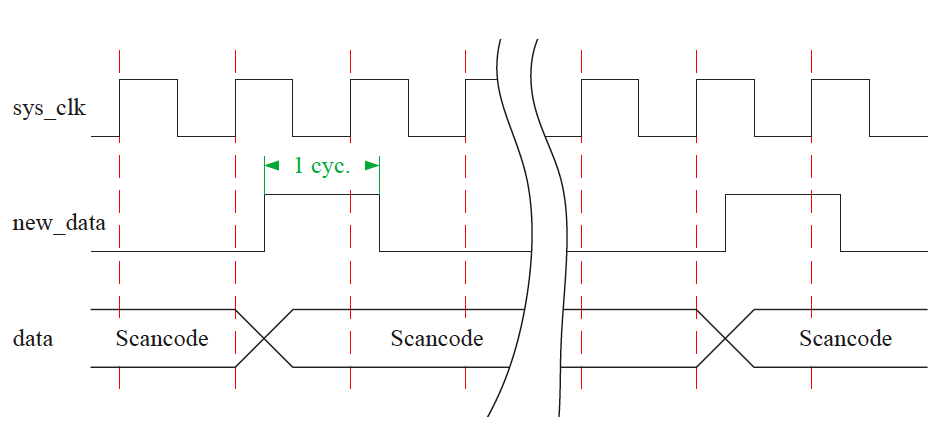
\includegraphics[scale=0.40]{figures/ps2_timing.png} 
	\caption{PS/2 Schnittstelle Timingdiagramm}
	\label{fig:ps2timing}
\end{figure}

Es muss also ein HIGH-Pegel auf new\_data anliegen, dann kann bei der nächsten steigenden Flanke der Systemclock ein neuer Scancode gelesen werden.
Die Scancodetabelle für eine Standard - PS/2 - Tastatur kann unter 
\par
http://www.computer-engineering.org/ps2keyboard/scancodes2.html

abgerufen werden. Für unsere Anwendung ist natürlich nur ein kleiner Teil davon von Interesse. Wir haben uns entschlossen als Eingabetasten nur die entsprechenden Numpad-Tasten zuzulassen, und zusätzlich noch die Leertaste, welche ja auch eine gültige Eingabe darstellt. Die erlaubten Eingaben plus Scancodes für MAKE und BREAK - Events können aus Tabelle~\ref{tab:scan_codes} entnommen werden:

\begin{table}[!h]
\begin{center}
\begin{tabular}{|l|l|l|}
\hline
Zeichen & Wait-Code & Break-Code\\
\hline
\hline

KP / & E0,4A & E0,F0,4A	\\
KP EN & E0,5A & E0,F0,5A \\
KP * & 7C & F0,7C \\
KP - & 7B & F0,7B \\
KP + & 79 & F0,79 \\
SPACE & 29 & F0,29 \\
BKSP & 66 & F0,66 \\
KP 0 & 70 & F0,70 \\
KP 1 & 69 & F0,69 \\
KP 2 & 72 & F0,72 \\
KP 3 & 7A & F0,7A \\
KP 4 & 6B & F0,6B \\
KP 5 & 73 & F0,73 \\
KP 6 & 74 & F0,74 \\ 
KP 7 & 6C & F0,6C \\ 
KP 8 & 75 & F0,75 \\
KP 9 & 7D & F0,7D \\
\hline
\end{tabular}
\end{center}
\caption{erlaubte Eingaben plus Scancodes für MAKE und BREAK}
\label{tab:scan_codes}
\end{table}

Prinzipiell müsste also die Logik, welche die ankommenden Scancodes auswertet und auf die den gedrückten Tasten entsprechenden ASCII-Werte mappt zuerst auf einen WAIT-Code warten und dürfte erst bei Erhalt des zugehörigen BREAK-Codes das entsprechende Zeichen abspeichern. Über die Zeitdifferenz zwischen WAIT - und BREAK-Code und einer frei zu wählenden Tastenwiederholungsrate könnte die Anzahl der zu speichernden Zeichen bestimmt werden. Damit würde die zugehörige State-Machine allerdings komplexer als notwendig werden. Wir haben uns deshalb dazu entschlossen, nur die BREAK-Code-Sequenzen der gewünschten Zeichen zu detektieren, und alle anderen ankommenden Codes zu ignorieren. Daraus ergibt sich natürlich 1. dass das Zeichen erst erkannt wird wenn die entsprechende Taste wieder losgelassen wird, und 2. dass - egal wie lange die Taste gedrückt wurde, immer nur ein einzelnes Zeichen erkannt wird. 
Sobald ein neues Zeichen erkannt wurde muss dieses natürlich in einem entsprechenden Buffer abgespeichert werden. Sobald ein <ENTER> - Zeichen erkannt wurde oder die maximale Eingabelänge erreicht wurde wird die Eingabe abgeschlossen.

Abbildung\ref{fig:scan}  zeigt die Funktionalität.

\subsubsection{Datenausgabe}

Die Ausgabe erfolgt per VGA, wobei dies von 2 verschiedenen Modulen realisiert wird: die eingegebenen Zeichen werden vom Scancode-Modul geschrieben - ist die Eingabe abgeschlossen(<ENTER> bzw. 70 Zeichen eingegeben) wird mittels ASCII-Char 'für <NEWLINE> in eine neue Zeile gewechselt und die Kontrolle an das Parser/Calculator-Modul übergeben. Dieses bestimmt das Ergebnis der aktuellen Eingabe und schreibt diese(bzw. eine Fehlermeldung bei falscher Syntax) an die aktuelle Position im VGA-Buffer. Danach wird wieder mittels <NEWLINE> in die nächste Zeile gewechselt und das Scancode-Modul übernimmt wieder die Kontrolle.

Folgende VGA-Commandos werden benötigt:

\begin{itemize}

\item COMMAND\_SET\_CURSOR\_COLUMN
\item COMMAND\_SET\_CURSOR\_LINE
\item COMMAND\_SET\_CURSOR\_COLOR
\item COMMAND\_SET\_CURSOR\_STATE
\item COMMAND\_SET\_CHAR
\end{itemize}

\subsection{Speichern von Rechnungen}

Es werden nur gültige Eingabelines gespeichert. Dazu wird nach erfolgter Eingabe vom Parser/Calculator-Modul das Ergebnis berechnet. Danach wird die eingegebene Zeile($Line\_buffer$, Index 0 bis $Line\_ptr$), gefolgt vom Delimiter '=' und dem Ergebnis in die aktuelle Position eines Ringbuffers mit der Grösse 50 x 81 Zeichen geschrieben Die Elementgrösse 81 des Arrays ergibt sich aus den max. 70 einzugegebenen Zeichen, dem Delimiter '=' und dem Ergebnis mit max. 10 Zeichen($2^{31}$).

\subsection{RS232 Schnittstelle}

Es muss sowohl Empfang als auch Senden von Datenbytes per Software-UART realisiert werden. Dazu muss ein Baudrate-Generator implementiert werden. Die Systemclock liefert ein Rechtecksignal mit f=33.33MHz - diese Frequenz muss geteilt werden, um eine gültige Baudrate erreichen zu können.

RS232 ist ein Standard für eine serielle Schnittstelle, wobei im Standard Timing, Spannungspegel, Leitungen und Stecker definiert sind.
Die Daten werden Bitseriell und asyncron übertragen, was in Abbildung~\ref{fig:rs232frame} dargestellt ist. Allerdings ist zu beachten dass RS-232 mit Signalpegeln im Bereich von +3 bis +15 V zur Darstellung einer logischen 0 (SPACE) und -3 bis -15 V zur Darstellung einer logischen 1 arbeitet.
 
\begin{figure}[!ht]
	\centering
	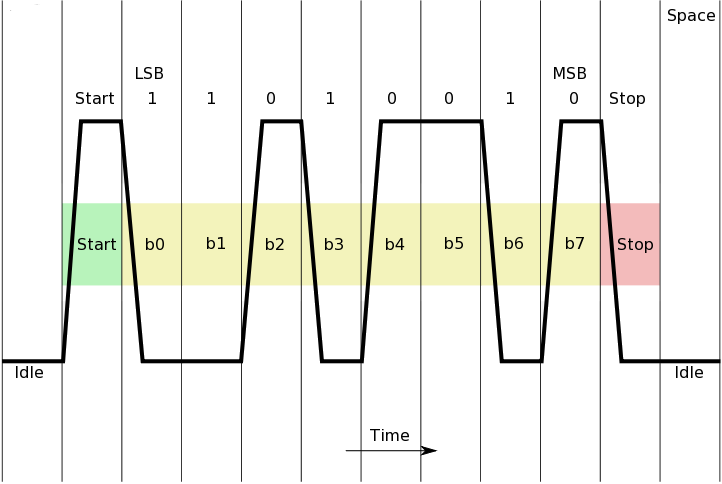
\includegraphics[scale=0.5]{figures/rs232Trace.png} 
	\caption{Datenframe RS232}
	\label{fig:rs232frame}
\end{figure}

Laut Angabe ist gefordert, die letzten 50 Berechnungen per RS232 versenden zu können, und dieser Sendevorgang soll auch per seriell empfangenen Zeichen angestossen werden können. Daraus folgt dass wir sowohl eine Sende- als auch eine Empfangsroutine für RS232 implementieren müssen. Als Triggerzeichen haben wir uns auf das Zeichen 's' geeinigt. Als Baudrate verwenden wir 38400 (Fehler aufgrund sys\_clk am geringsten), als Format 8N1(8 Datenbits, No Paritiy, 1 Stopbit).

Der Teiler berechnet sich mittels $divisior = \frac{Sys\_clk}{Baudrate}$ - Tabelle~\ref{tab:baudrates} zeigt die Einstellmöglichkeiten.


\begin{table}[!h]
\begin{center}
\begin{tabular}{|l|l|l|}
\hline
Baudrate  & Teiler\\
\hline
\hline

2400 & 13887.5 \\ 
 4800 & 6943.75\\
 9600 & 3471.875\\
 19200 & 1735.9375 \\
 38400 & 867.96875 \\
 57500 & 578.6458 \\
 115200 & 289.32 \\
 
\hline
\end{tabular}
\end{center}
\caption{mögliche Baudrates}
\label{tab:baudrates}
\end{table}

\section{Detailierte Design Beschreibung der Module}

\begin{figure}[!ht]
	\centering
	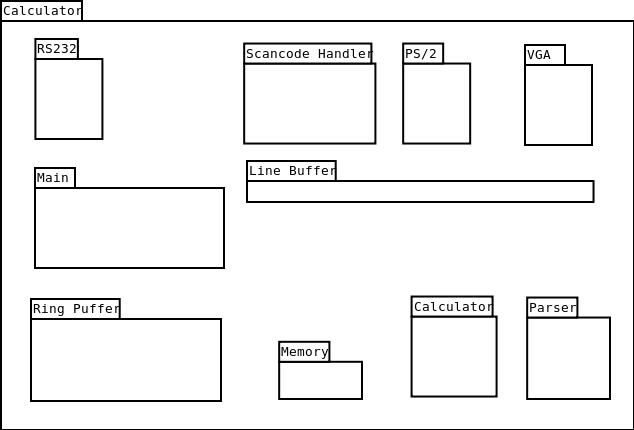
\includegraphics[scale=0.5]{figures/mod_view.png} 
	\caption{Modularer Aufbau der Applikation}
	\label{fig:mod_view}
\end{figure}

\subsection{Main}

\begin{figure}[!ht]
	\centering
	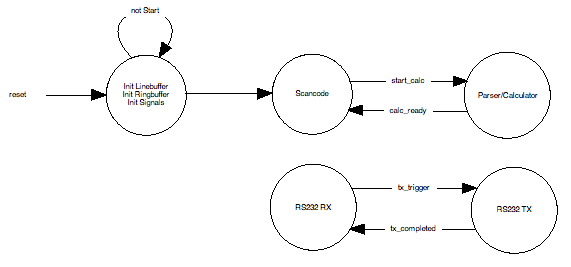
\includegraphics[scale=0.5]{figures/mainSM.png} 
	\caption{Benötigte Programmmodule}
	\label{fig:mainSM}
\end{figure}

Das Programm setzt sich aus dem Scancode-Handler-Modul, dem RS232-Modul(Senden und Empfangen), einem Ringbuffer Modul, einem Line Buffer Modul, Memory Modul sowie dem Parser/Calculator-Modul zusammen, siehe Abbildung~\ref{fig:mainSM}. 
Die beiden Puffer instanzieren dabei das Modul Memory.

Beim Einschalten wird ein Reset/Init sämmtlicher verwendeter Speicher durchgeführt. Danach beginnt die Programmausführung mit dem Scancode-Modul, parallel dazu schaltet das RS232-Modul in Empfangsmodus - diese 2 Module werden laufen also parallel ab.

Die Main ist die zentrale Steuereinheit des gesammten Programms. Sie aktiviert bzw. deaktiviert (Signal 'enable') den Line Buffer sowie das Calculator Modul. Der Zugriff auf die beiden Speicherbereiche (Lien Buffer und Ringbuffer) sowie die Kommunikation mit dem RS232 Modul wird ebenfalls vom Main Modul geregelt.


\subsection{Scancode Handler}

\begin{figure}[!ht]
	\centering
	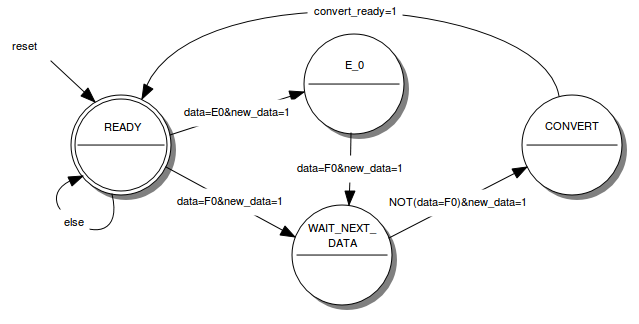
\includegraphics[scale=0.4]{figures/scancode.png} 
	\caption{Statemachine für das Scancode Handler Modul}
	\label{fig:scan}
\end{figure}


In Abbildung\ref{fig:scan}  ist die Funktionalität des Scancode-Moduls abgebildet:

Zuerst werden die verwendeten Puffer und Signale resettet/initialisiert. Danach wird in 'READY' auf eine steigende Flanke von $data\_new$ gewartet. Wenn diese auftritt wird überprüft ob das empfangene Byte hexadezimal gleich F0 oder E0 ist. Ist es gleich F0 wird sofort in den Zwischenzustand 'WAIT\_NEXT\_DATA' gewechselt. Da wir die Breakcodes der Zeichen auswerten, ist im Zustand 'E\_0' das nächste eingelesene Byte, hexadezimal immer F0. Dieses wird bei der nächsten steigenden Flanke von $data\_new$ einfach ignoriert und ebenfalls in den Zustand 'WAIT\_NEXT\_DATA' gewechselt.
Diesen Zustand haben wir eingefürht da es möglich ist, dass das nächste Zeichen vom PS2 Modul noch nicht zur Verfügung steht obwohl bereits die steigende Flanke von $data\_new$ erkannt wird.
Nur wenn das eingelesene Byte nicht F0 ist, wird in den Zustand 'CONVERT' gewechselt und das entsprechende Ascii Zeichen am Ausgang bereit gestellt sowie der Port $new\_ascii$ gesetzt. Dadurch wird signalisiert, dass ein neues Zeichen eingelesen wurde und zur weiterverarbeitung bereit steht.  


\subsection{Parser (Scancode Handler Puffer einlesen \& interpretieren)}

Abbildung~\ref{fig:parser} zeigt eine Statemachine für den Parser, in Abbildung~\ref{fig:entity_parser} sind die Ein- und Ausgänge des Moduls dargestellt (Entity). Der Parser wird vom Calculatormodul verwendet um den mathematischen Ausdruck welchen der Scancodehandler in einem Puffer (70 Zeichen Puffer) in Form von Ascii Zeichen zur Verfügung stellt auszuwerten und zu interpretieren. \\
Im Folgenden wird die Funktionalität der Parser Statemachine sowie die Abläufe inerhalb der einzelnen States genauer beschrieben.

\begin{figure}[!ht]
	\centering
	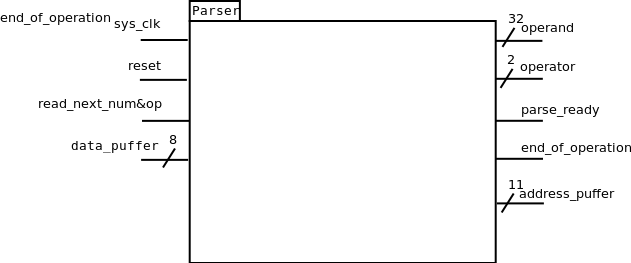
\includegraphics[scale=0.5]{figures/entity_parser.png} 
	\caption{Entity des Parsers}
	\label{fig:entity_parser}
\end{figure}

\begin{figure}[!ht]
	\centering
	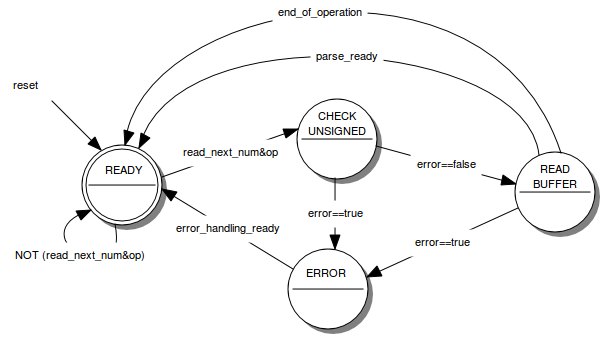
\includegraphics[scale=0.5]{figures/parser.png} 
	\caption{Statemachine für das Modul Parser}
	\label{fig:parser}
\end{figure}

\begin{itemize}

\item State: READY (Initial- und Endzustand) \\
Vom Calculatormodul wird mittels dem Signal read\_next\_num\&op der nächste/erste Operand und Operator angefordert. \\ 
Die Statemachine bleibt im READY Zustand solange keine neue Anforderung vom Calculatormodul kommt.

\item State: CHECK UNSIGNED \\
Sobald vom Calculatormodul eine neue Zeichenauswertung angefordert wird wechselt die Statemachine in den Zustand CHECK UNSIGNED. In diesem Zustand wird überprüft ob der nächste Operand vorzeichenbehaftet ist.
Der Ablauf in diesem State kann wie folgt beschrieben werden. \\
Zuerst wird das nächste Zeichen geprüft, ist dieses Zeichen eine Ziffer von 0 bis 9 wird der Puffer Positionspointer nicht incrementiert und sofort in den Zustand READ BUFFER gewechsetl. \\
Ist das nächste Zeichen kein Minus und auch keine Ziffer von 0 bis 9, so liegt ein ungültiger mathematischer Ausdruck vor und es wird in den Zustand ERROR gewechselt. \\
Ist das nächste Zeichen ein Minus, wird der Positionspointer um eins incrementiert und das nächste Zeichen überprüft. Wenn dieses Zeichen nun eine Ziffer von 0 bis 9 ist, wird das Signal 'leading\_sign' gesetzt welches anzeigt, dass der nächste Operand vorzeichenbehaftet und in den Zustand READ BUFFER gewechselt. \\
Ansonst wird in den Zustand ERROR gewechselt.

\item State: ERROR \\
In diesem Zustand wird eine Next Line Command an das VGA Modul geschickt, danach die Fehlermeldung 'ungültiger mathematischer Ausdruck' in den VGA Puffer geschrieben und nochmal ein Next Line Command gesendet.
Danach wird vom Parser das Calculatormodul resetet und die Statemachine kehrt wieder in den Zustand READY zurück.

\item State: READ BUFFER \\
In diesem Zustand wird zuerst der aktuelle Wert des Pufferpointers (der Werd des Puffer Pointers wird vom Parser intern gespeichert un bei einem Reset mit 0 initialisiert) in einer Variablen (im folgenden pos\_var genannt) zwischengespeichert. Anschließend wird mit Hilfe dieser Variablen der Puffer so weit durchlaufen bis ein Leerzeichen bzw. ein Operator auftritt oder das Pufferende erreicht wird. Aus der Differenz vom aktullen Wert der Variablen pos\_var und dem Puffer Pointer Wert kann ermittelt werden, ob es sich um einen gültigen Operanden handelt (zu viele Stellen => zu großer nummerischer Wert). Diese Überprüfung wird immer ausgeführt nachdem das Ende eines Operanden erkannt wurde. Ist der Operand zu groß wird in den ERROR Zustand gewechselt. 

\begin{itemize}
\item Tritt ein Leerzeichen oder mehrere Leerzeichen hintereinander auf, muss überprüft werden ob das nachfolgende Zeichen eine Ziffer oder ein Operator ist. Handelt es sich um eine Ziffer so wird in den ERROR State gewechselt, handelt es sich um einen Operator wird dieser zwischengespeichert sowie die bisher eingelesenen Ziffer umgewandelt und ebenfalls zwischengespeichert. Falls das Signal 'leading\_sign gesetzt ist muss der umgewandelte Wert mittels Zweierkomplement vor der Speicherung in seine negative Darstellung gebracht werden. Danach kann 'leading\_sign' wieder deaktiviert werden. \\
Um welchen Operator es sich handelt wird mittles 2 Bit unterschieden. Die Zuteilung der Bitkombinationen zu den Operatoren is in Tabelle ~\ref{tab:operator_code} dargestell.
\item Tritt beim Pufferdurchlauf ein Operator auf, so hat man das Ende des nächsten Operanden ermittelt. Der Operator kann sofort zwischengespeichert werden. Handelt es sich um einen gültigen Operanden werden die Zifferen in einen Integer Wert umgewandelt und dieser Wert zwischengespeichert. Falls das Signal 'leading\_sign gesetzt ist muss der umgewandelte Wert mittels Zweierkomplement vor der Speicherung in seine negative Darstellung gebracht werden. Danach kann 'leading\_sign' wieder deaktiviert werden. 
\item Erreicht man beim Pufferdurchlauf das Ende des Puffers (pos\_var >=70) werden die bisher eingelesenen Ziffern umgewandelt und zwischengespeichert. Falls das Signal 'leading\_sign gesetzt ist muss der umgewandelte Wert mittels Zweierkomplement vor der Speicherung in seine negative Darstellung gebracht werden. Danach kann 'leading\_sign' wieder deaktiviert werden. \\
Mit dem Signal 'parse\_ready' kehrt der Parser in den READY State zurück, zusätzlich wird einerseits das Signal 'end\_of\_operation' aktiviert und somit der Calculator über das Ende der Rechnung informiert, andererseits muss der Puffer Pointer zurückgesetzt werden (um bei einer neuen Rechnung wieder von Anfang an lesen zu können) und der Puffer mit Leerzeichen gefüllt werden (damit auch beim nicht Ausnutzen des gesammten Puffers das Ende einer Rechnung erkannt wird). 
\end{itemize}

Nach erfolgreicher Zwischenspeicherung von Oerator und Operand kann in den Zustand READY gewechselt werden.  
\end{itemize}

\begin{table}[!h]
\begin{center}
\begin{tabular}{|l|l|}
\hline
Operator & Bit-Code\\
\hline
\hline

+ & 00 \\
- & 01 \\
* & 10 \\
/ & 11 \\
\hline

\end{tabular}
\end{center}
\label{tab:operator_code}
\caption{Zuweisung der Bitkombinationen zu den Operatoren} 
\end{table}

\subsection{Calculator}

Die Aufgabe des Calculatermoduls ist es mittels des Modules Parser immer einen Operanden und einen Operator einzulesen und diese richtig zu verarbeiten. Das Calculatormodul verwendet dazu 4 Speicherbereiche (wie in Abbildung~\ref{fig:vier_puffer} dargestellt). Damit wird je ein Operator und ein Operand für die Punktrechnung sowie für die Strichrechnung gespeichert.\\
Für die Operanden ist dabei ein 64 Bit Puffer vorgesehen, für die Operatoren ein 2 Bit Puffer.\\
Das Funktionsprinzip wird im folgenden an der State Machine (siehe Abbildung~\ref{fig:calculator}) erläutert, in Abbildung~\ref{fig:entity_calc} sind die Ein- und Ausgänge des Moduls dargestellt (Entity).

\begin{figure}[!ht]
	\centering
	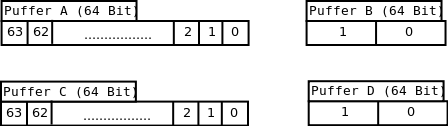
\includegraphics[scale=0.5]{figures/vier_puffer.png} 
	\caption{Puffer die das Calculator Modul verwendet}
	\label{fig:vier_puffer}
\end{figure}

\begin{figure}[!ht]
	\centering
	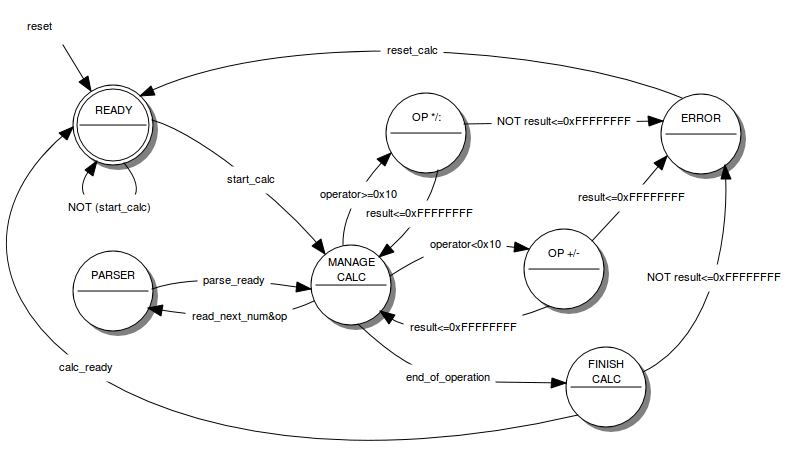
\includegraphics[scale=0.5]{figures/Calculator.png} 
	\caption{Statemachine für das Modul Calculator}
	\label{fig:calculator}
\end{figure}

\begin{figure}[!ht]
	\centering
	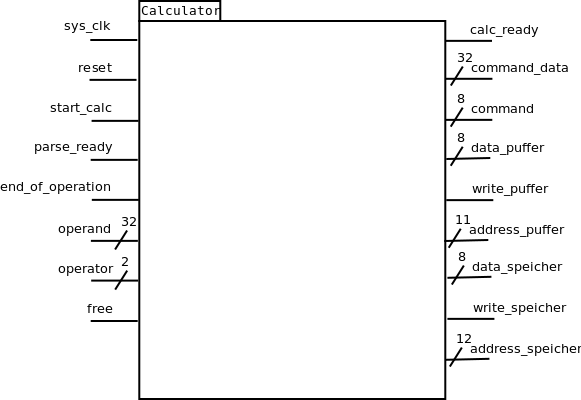
\includegraphics[scale=0.5]{figures/entity_calculator.png} 
	\caption{Entity des Calculatormodules}
	\label{fig:entity_calc}
\end{figure}

\begin{itemize}

\item State: READY \\
Der Anfangs und Endzustand des Moduls ist der READY State. Das Modul verharrt in diesem Zustand solange nicht durch das Signal 'start\_calc' eine neue Berechnung angestoßen wird. Es kehrt wieder in diesem Zustand zurück, wenn eine Berechnung abgeschlossen ist (letzter Operand verarbeitet ... wird durch Signal 'clac\_ready' angezeit) oder es z.B. aufgrund eines Fehlers resetet wird.

\item State: MANGAGE CALC \\
Wird eine neue Berechnung gestartet wechselt das Calculatormodul in den MANAGE CALC Zustand. Dies ist der zentrale Zustand für die gesammte Berechnung. Aus diesem Zustand heraus werden nächster Operator und Operand angeforder (Anforderung: Signal 'read\_next\_num\&op', OP und NUM vorhanden: Signal 'parse\_ready'), sowie überprüft ob es sich beim gerade eingelesenen Operator um einen Punktrechnungs- oder einen Strichrechnungsoperator handelt. Je nach Operatortyp wird dann entweder in den Zustand 'OP\_+/-' oder in den Zustand 'OP\_*/:' gewechselt. \\
Ist zusätzlich das Signal 'end\_of\_operation' aktiv wird in den Zustand FINISH CALC gewechselt und die Berechung abgeschlossen.


\item State: PARSER \\
Wenn das Modul im Zustand MANAGE CALC ist kann es mit Hilfe des Parsers einen neuen Operator und Operanden anfordern (Signal 'read\_next\_num\&op). Das Modul wechselt in den State PARSE und verharrt dort bis die Anforderung abgearbeitet ist. Durch das Signal 'parse\_ready' wird angezeigt, dass ein neuer Operand sowie ein (optionaler) neuer Operator zur Verarbeitung bereit stehen, es wird wieder in den MANAGE CALC State gewechselt. 

\item State: OP\_*/: \\
In diesem State muss zuerst überprüft werden, ob bei einem vorliegende Divisionsoperator eine 0 als Operand eingelesen wurde (Division durch 0). Ist dies der Fall wird sofort in den ERROR State gewechselt. Ist dies nicht der Fall kann zwischen 2 möglichen Szenarien unterschieden werden.
Die Pufferbezeichnungen A, B, C und D beziehen sich auf Abbildung~\ref{fig:vier_puffer}.

\begin{enumerate}

\item Falls noch keine Operation vorgemerkt ist, wird der Operand in einem 64 Bit Puffer (Puffer A) gespeichert und er Operator in einem 2 Bit Puffer (Puffer B). \\

\item Ist jedoch bereits eine Operation vorgemerkt, wird der vorgemerkte Operand (Puffer A), abhängig vom vorgemerkten Operator (Puffer B), mit dem aktuellen Operanden verarbeite (Berechnung wird durchgeführt) und in Puffer A gespeichert. \\
Danach wird überprüft ob der Wert im 64 Bit Puffer (Puffer A) kleiner oder gleich 0xFFFFFFFF. Ist dies der Fall, ist das Ergebnis mit einer 32 Bit Variablen darstellbar und der Aktuelle Operator kann in Puffer B gespeichert werden. \\
Ist dies nicht der Fall, wird sofort in den ERROR State gewechselt. 

\end{enumerate}

\item State: OP\_+/- \\
In diesem State muss zwischen 4 möglichen Startszenarien unterschieden werden.
Die Pufferbezeichnungen A, B, C und D beziehen sich auf Abbildung~\ref{fig:vier_puffer}.

\begin{enumerate}

\item Es ist weder eine Punktrechnung, noch eine Strichrechnung gespeichert (alle 4 Puffer sind 0)\\
In diesem Fall wir der Operand in Puffer C gespeicher und der Operator in Puffer D.

\item Es ist keine Punktrechnung gespeichert jedoch bereits eine Strichrechnung (Puffer A und Puffer B sind 0, Puffer C und Puffer D sind ungleich 0) \\
In diesem Fall wird genau wie im vorigen Szenarion vorgegangen.

\item Es ist bereits eine Punktrechnung gespeichert, jedoch keine Strichrechnung (Puffer A und Puffer B sind ungleich 0, Puffer C und Puffer D sind 0)\\
Bei diesem Szenario muss zuerst überprüft werden ob bei einem vorliegende Divisionsoperator eine 0 als Operand eingelesen wurde. Ist dies der Fall, wird sofort in den ERROR State gewechselt. Andernfalls wird der vorgemerkte Operand (Puffer A), abhängig vom vorgemerkten Operator (Puffer B), mit dem aktuellen Operanden verarbeite (Berechnung wird durchgeführt) und in Puffer C gespeichert. \\
Danach wird überprüft ob der Wert im 64 Bit Puffer (Puffer C) kleiner oder gleich 0xFFFFFFFF. Ist dies der Fall, ist das Ergebnis mit einer 32 Bit Variablen darstellbar und der Aktuelle Operator kann in Puffer D gespeichert werden. \\
Puffer A und Puffer B müssen gelöscht werden (logische Und- Verknüpfung mit 0)

\item Es ist sowohl eine Punktrechnung als auch eine Strichrechnung vorgemerkt (Alle 4 Puffer sind ungleich 0) \\
Hier muss zuerst wieder überprüft werden, ob eine Division durch 0 vorliegt. Ist in Puffer B ein Divisionsoperator gespeichert und der aktuelle Operand gleich 0 so wird sofort in den ERROR State gewechselt. Andernfalls wird der vorgemerkte Operand (Puffer A) abhängig vom vorgemerkten Operator (Puffer B), mit dem aktuellen Operanden verarbeite (Berechnung wird durchgeführt) und in Puffer A zwischengespeichert. An dieser Stelle muss das Ergebnis wieder dahingehend überprüft werden ob es noch kleiner 0xFFFFFFFF ist und entweder die Berechnung fortgesetzt oder in den ERROR State gewechselt werden. Danach wird der Operand von Puffer A abhängig vom Operator von Puffer D mit dem Operanden von Puffer C verarbeitet und in Puffer C gespeichert.\\ 
Nun wird wieder überprüft ob der Wert im 64 Bit Puffer (Puffer C) kleiner oder gleich 0xFFFFFFFF. Ist dies der Fall, ist das Ergebnis mit einer 32 Bit Variablen darstellbar und der Aktuelle Operator kann in Puffer D gespeichert werden. \\
Weiters müssen Puffer A und Puffer B gelöscht werden (logische Undverknüpfung mit 0).

\end{enumerate}

\item State: FINISH\_CALC \\
Falls das Signal 'end\_of\_operation' aktiv ist, wird vom Zustand MANAGE CALC in den Zustand FINISH CALC gewechselt. \\
In diesem Zustand wird zuerst überprüft ob eine Punktrechnung vorgemerkt ist (Puffer B ungleich 0). Ist dies der Fall, wird auf eine mögliche Division durch 0 geprüft und falls nötig in den ERROR State gewechselt. Wird nicht in den ERROR State gewechselt muss die Punktrechnung durchgeführt werden und falls auch eine Strichrechnung vorgemerkt ist, diese auch abgearbeitet werden. \\
Sind alle Berechnungen abgeschlossen wird das Ergebnis wieder in Asciizeichen umgewandelt und zeichenweise in den VGA Puffer (warten bis VGA Modul frei... Signal 'free', in den VGA Puffer schreiben ... Signal 'command\_data' und 'command', siehe Abbildung~\ref{fig:entity_calc}) sowie der gesamte $Line\_buffer$ in den Ringspeicher ('write' Signal, 'addres' Signal und Datenbus 'data', siehe Abbildung~\ref{fig:entity_calc}) geschrieben. 
Das Signal 'calc\_ready' wird aktiviert und das Calculatormodul kehrt wieder in den Zustand READY zurück. 

\item State: ERROR \\
In diesem Zustand wird eine Next Line Command an das VGA Modul geschickt, danach die Fehlermeldung 'Bufferoverflow' in den VGA Puffer geschrieben und nochmal ein Next Line Command gesendet.
Danach wird das Calculatormodul resetet und die Statemachine kehrt wieder in den Zustand READY zurück.

\end{itemize}

\subsubsection{Addition}

Die Addier-Funktionalität wird mittels Addierer realisiert, hier muss von unserer seite her kein spezieller Aufwand betrieben werden.
Wenn in VHDL eine Anweisung der Form ERG = Z1 + Z2 vorkommt erzeugt der Compiler eine entspr. Addierschaltung mit n Bit, wobei hier n der Bitbreite von Z1 und Z2 entspricht.

\subsubsection{Subtraktion}

Hier gilt das gleich wie bei der Addition, nur dass hier natürlich eine Subtrahierschaltung anstatt einer Addierschaltung erzeugt wird.

\subsubsection{Multiplikation}

Siehe oben.

\subsubsection{Division}

Die Divion bildet einen Sonderfall unter den geforderten Rechenoperationen. Prinzipiell könnte diese Rechenoperation - wie bei den 3 vorhergehenden - einfach über die Anweisung ERG = Z1 / Z2 abgebildet werden. Die resultierende Schaltung wäre aufgrund der relativ hohen Bitbreite allerdings sehr komplex, wodurch der kritische Pfad sehr lange werden würde, damit verbunden würde diese Schaltung dann einen entsprechend hohen Delay verursachen. Die Dividier-Operation wird also von einer eigens implementierten Algorithmus realisiert. 

\subsection{Ringpuffer}

Im Ringpuffer (siehe Abbildung~\ref{fig:entity_ring}) werden die letzten 50 gültigen Rechenoperationen inklusive Ergebnisse gespeichert. Zum schreiben auf den Puffer muss das 'write\_speicher' Signal aktiviert werden. Zusätzlich muss am Address Port (Signal'address\_speicher') die gewünschte Adresse sowie am Dateneingang (Signalbus 'input\_speicher') das zu speichernde Byte angelegt werden.

\begin{figure}[!ht]
	\centering
	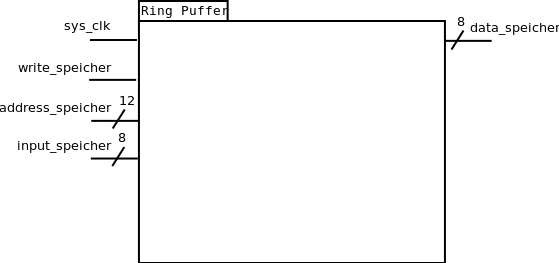
\includegraphics[scale=0.5]{figures/entity_speicher.png} 
	\caption{Entity Ringpuffer}
	\label{fig:entity_ring}
\end{figure}

\subsection{Line Buffer}

Der Line Buffer ist dafür zuständig die aktuell eingegebene Rechnung zwischen zu speichern. Dafür wird das Memory Modul (für die eigentliche Zwischenspeicherung) sowie das PS2 Modul und das Scancode Handler Modul (für die Eigabe der Zeichen) verwendet. Eine weitere Aufgabe des Line Buffers ist es, die eingelesenen Zeichen mit Hilfe des VGA Moduls am Bildschirm darzustellen. Die dafür benötigte Statemachine ist in Abbildung ~\ref{fig:fsm_lb} dargestellt. 

Um die Zeichen ENTER und BACKSPACE richtig darzustellen, müssen dem VGA Modul mehr als nur ein Zeichen übergeben werden (ENTER: linefeed und nextline, BKSP: Cursorposition um eins verrigern, Leerzeichen schreiben und Cursorposition wieder um eins verringern). Wenn für das Schreiben eines Zeichens mehr als ein VGA Befehl benötigt wird braucht man einen Zwischenzustand (WAIT\_STATE), da das VGA Modul eine gewisse Zeit braucht um ein Zeichen auf dem Bildschirm abzubilden.
Da bei einem Reset der VGA Speicher nicht gelöscht wird, haben wir zusätzlich noch den Zustand CLEAR\_SCREEN eingeführ. In diesem Zustand wird 30 mal ein nextline Befehl dem VGA Modul übergeben um bei einem Reset den Bildschirm zu leeren. Danach wird in den eigentlichen Startzustand CHECK\_ASCII gewechselt.
Die Ein- und Ausgänge des Moduls sind in Abbildung~\ref{fig:entity_buffer} zu finden. 
Mit Dem Signal 'read\_ready' signalisiert der Line Buffer das eine Eingabe abgeschlossen ist und zur weiterverarbeitung (Berechnung) bereit steht. Durch den Eingangsport 'enable' kann der Linebuffer abgeschaltet werden. Dies ist wichtig, da während der Auswertung des einglesenen Ausdrucks dieser nicht verändert werden darf. Erst wenn die Berechnung abgeschlossen ist, darf der Line Buffer wieder Zeichen einlesen. Sobald der Port 'enable' auf 1 gesetzt wird, wird der Speicher mit Leerzeichen überschrieben und der Linebuffer kehrt in den Zustand 'CHECK\_ASCII' zurück.

\begin{figure}[!ht]
	\centering
	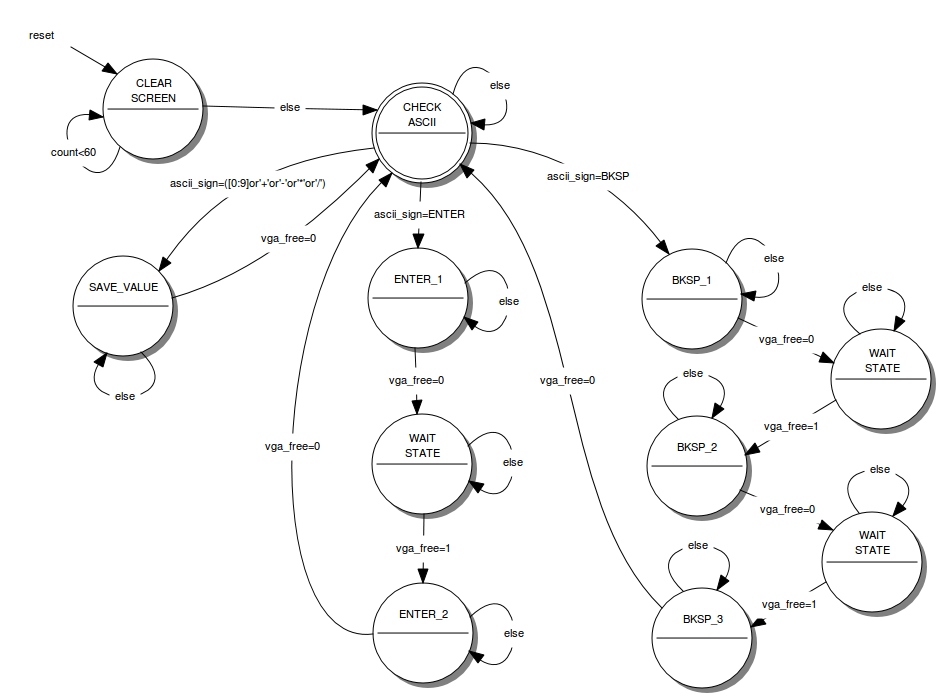
\includegraphics[scale=0.40]{figures/line_buffer.png} 
	\caption{State Machine Line Buffer}
	\label{fig:fsm_lb}
\end{figure}

\begin{figure}[!ht]
	\centering
	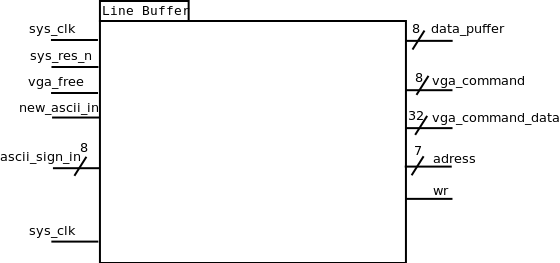
\includegraphics[scale=0.5]{figures/entity_puffer.png} 
	\caption{Entity Line Buffer}
	\label{fig:entity_buffer}
\end{figure}


\subsection{Externe Schnittstellen}

Hardware spezifisches zu den Schnittstellen, + Logische Implementierung

\subsubsection{RS232-Schnittstelle}

\begin{figure}[!ht]
	\centering
	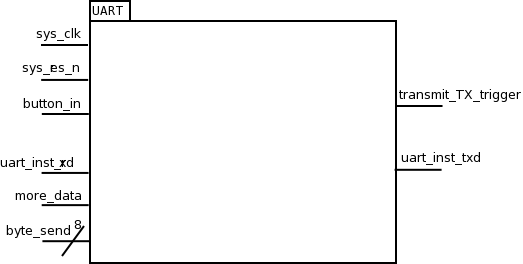
\includegraphics[scale=0.3]{figures/uart.png} 
	\caption{Entity der UART Hauptinstanz}
	\label{fig:entity_rs232}
\end{figure}

\begin{figure}[!ht]
	\centering
	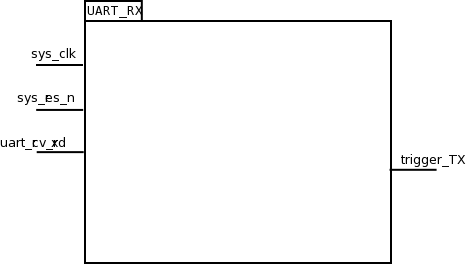
\includegraphics[scale=0.3]{figures/uart_rx.png} 
	\caption{Entity der UART-Empfangsinsanz}
	\label{fig:entity_rs232_rx}
\end{figure}

\begin{figure}[!ht]
	\centering
	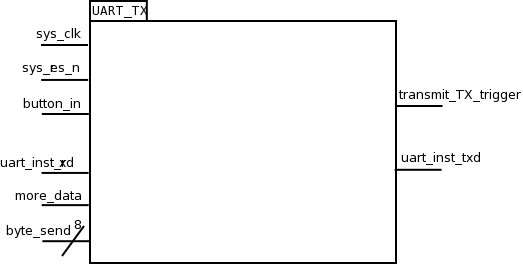
\includegraphics[scale=0.3]{figures/uart_tx.png} 
	\caption{Entity der UART-Sendeinstanz}
	\label{fig:entity_rs232_tx}
\end{figure}

In Abbildung~\ref{fig:rs232statemachine} ist die Statemachine des RS232 Moduls zu sehen, Abbildung~\ref{fig:entity_rs232} zeigt Ein- und Ausgänge der Hauptinstanz. Die UART-Funktionalität ist modular aufgebaut, zusätzlich zur UART-Hauptinstanz gibt es die Unterinstanzen UART\_RX~\ref{fig:entity_rs232_rx} und UART\_TX~\ref{fig:entity_rs232_tx} . Die Funktionalität wird im Folgenden beschrieben. \\
Wenn das Board neu gestartet wurde werden zuerst die Buffer für Sende/Empfangsroutinen initialisiert. Danach muss die Empfangsroutine aktiviert werden. Dazu muss ein Baudrategenerator gestartet werden, welcher, sobald ein START-Bit erkannt wurde(wechsel von IDLE/negativer Spannungspegl = logische HIGH auf positiven Pegel), immer möglichst genau in der Mitte der zu empfangenden Bits den aktuellen logischen Pegel auf der RX-Leitung  einliest und in einen Buffer speichert(LSB wird immer als erstes gesendet). Danach muss noch ein gültiges STOP-Bit gelesen werden(negativer Spannungspegel). Jetzt muss noch geprüft werden ob dieses eingelesene Byte mit dem Triggerzeichen(bei uns 's') übereinstimmt. Falls ja wird die Main-Instanz per Signal verständigt dass das Triggerzeichen empfangen wurde. Gleiches gilt wenn das Signal für den 'pushbutton' aktiviert wird(Taste muss entprellt werden). Während eines Sendevorgangs können keine Zeichen eingelesen werden, diese Routine 'blockiert' also.
Wenn also ein Sendevorgang angestossen wurde versorgt die Main-Instanz das UART-Modul(und in weiterer Folge das UART-TX-Modul) mit den einzelnen Bytes aus der Memory-Instanz(wo die fertigen Berechnungen gespeichert werden). Dazu kopiert zuerst die Main-Instanz das 1. zu sendende Byte in 'byte\_out' und setzt das Steuersignal 'more\_data' auf HIGH(dieses bleibt HIGH solange Bytes zu senden sind). UART\_TX setzt nun das Signal 'tx\_busy' und schreibt das Byte auf die Serielle Schnittstelle, sobald die Leitung wieder auf IDLE gesetzt wurde wird 'tx\_busy' auf LOW gesetzt. Dies ist das Zeichen für die Main-Instanz, das nächste Zeichen aus dem Speicher zu holen usw.  


Eine Zeile wird mittels Newline 0x0A und Carriage Return 0x0D abgeschlossen, diese Sonderzeichen sind nicht im Speicher sondern müssen von der Main-Instanz extra eingefügt werden. Weiters haben wir beschlossen, sobald ein Sendevorgang angestossen wurde, immer den gesamten Ringbuffer(also alle 50 Zeilen zu je max. 80 Zeichen) zu senden, egal wieviele Berechnungen bisher gespeichert wurden.

\begin{figure}[!ht]
	\centering
	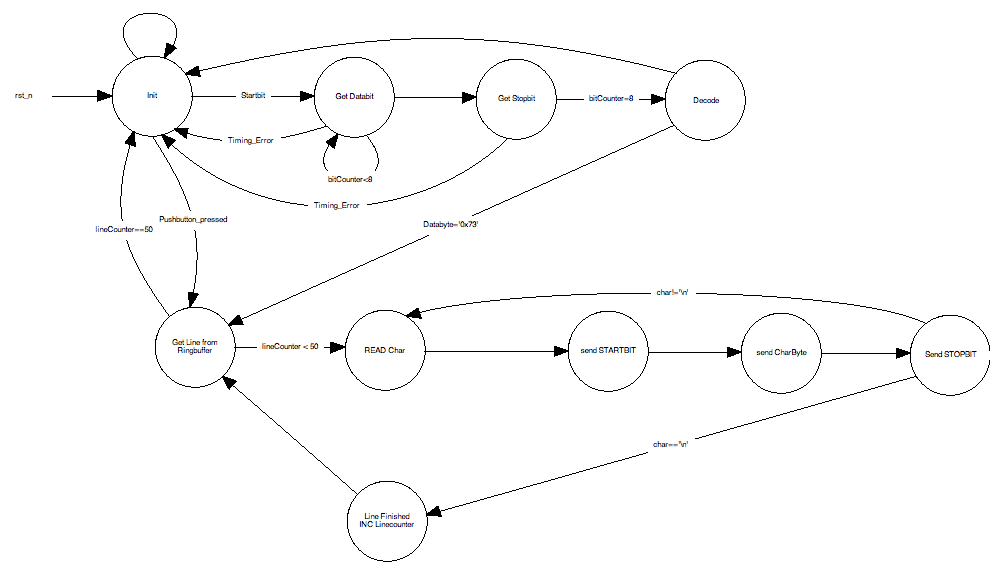
\includegraphics[scale=0.3]{figures/rs232SM.png} 
	\caption{Statemachine für Sende- und Empfangsroutine}
	\label{fig:rs232statemachine}
\end{figure}



\subsubsection{PS/2-Schnittstelle}

Es wird ein Modul von der LVA-Leitung zur Verfügung gestellt welche die Kommunikation Keyboard-Controller / FPGA-Board übernimmt (Abbildung~\ref{fig:entity_ps2} zeigt die Entity es Moduls). Unsere Aufgabe ist es die ankommenden Scancodes auszulesen und auf die entsprechenden ASCII - Codes zu mappen. Siehe Kapitel 'Scancode - Handler'.

\begin{figure}[!ht]
	\centering
	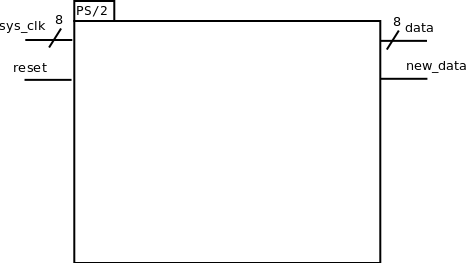
\includegraphics[scale=0.3]{figures/entity_ps2.png} 
	\caption{Entity des PS/2 Moduls}
	\label{fig:entity_ps2}
\end{figure}

\subsubsection{VGA-Schnittstelle}

Wie gesagt wird ein Modul zur Ansteuerung eines VGA-Monitors von der LVA-Leitung zur Verfügung gestellt (Abbildung~\ref{fig:entity_vga} zeigt die Entity es Moduls). Dieses Modul unterstützt Standard-VGA-Modus, also eine 'Auslösung' von 80 Zeichen pro Zeile, und 30 derartige Zeilen. Als Zeichensatz wird die 'Western European Codepage CP850' unterstützt, womit alle gängigen ASCII-Zeichen dargestellt werden können.

Hintergrundfarbe, Textfarbe und Cursorform können frei gewählt werden, wobei eine Farbauslösung laut Standard-VGA von 8Bit unterstützt wird. Um einen möglichst hohen Kontrast und damit beste Lesbarkeit zu erzielen verwenden wir weissen Text auf schwarzem Hintergrund. Cursorfarbe ist weiss blinkend.
Die Textausgabe startet in der 1. Zeile, 5. Zeichen, mit einem blinkenden Cursor. Eingegebene Zeichen werden in einen Buffer geschrieben, und dieser Buffer wird laufend von unserem sync\_ps2tovga - Modul mittels dem Kommando 'COMMAND\_SET\_CHARACTER' in den VGA-Speicher geschrieben. Sobald die Eingabe abgeschlossen 	ist(entweder mit Eingabe von 'ENTER' oder nach der Erreichen der laut Angabe maximal 70 eingelesenen Zeichen) springt der Cursor in die nächste Zeile und gibt ab x-Position 10 das Ergebnis oder, im Falle einer falschen Eingabesyntax, den Text \textbf{'Fehlerhafte Eingabe'} aus. Um den Cursor zu positionieren können in x-Richtung Leerzeichen und in y-Richtung 'CL/LF' verwendet werden, es gibt aber auch spezielle Kommandos um den Cursor an eine beliebige Stelle setzen zu können.

Siehe auch Kapitel 'Scancode - Handler' bzw. 'Calculator'.

\begin{figure}[!ht]
	\centering
	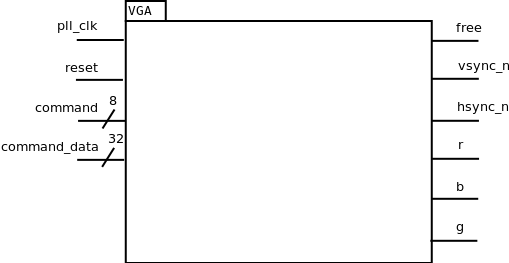
\includegraphics[scale=0.3]{figures/entity_vga.png} 
	\caption{Entity des VGA Moduls}
	\label{fig:entity_vga}
\end{figure}

\section{Testfälle}

\begin{itemize}

\item Eingabe von nicht definierten Zeichen - müssen ignoriert werden
\item Eingabe von zu grossen Zahlen als Operator( $z > 2^{31}$)  - Fehlermeldung
\item Eingabe von Leerzeichen innerhalb von Zahlen - Fehlermeldung
\item Eingabe von mehreren Operatoren zwischen 2 Zahlen(Ausnahme: negativ-Zeichen  - Fehlermeldung
\item Division durch Null - Fehlermeldung
\item Eingabe von zu vielen Zeichen - Abbruch der Eingabe nach 70 Zeichen, Berechnung dieses Ausdrucks
\item Triggern eines UART\_TX per UART\_RX
\item Triggern eines UART\_TX per Pushbutton

\end{itemize}


\end{document}
